% Expression Atlas section template
\subsection{Expression Atlas: independent RNA-seq tissue specificity}
\label{sec:eatlas}
ProteomicsDB found gated proteins in more normal tissues than background.
We tested whether an independent RNA-seq atlas reproduces RNA-level
restriction, using EBI Expression Atlas baseline experiment
E-MTAB-513 (Illumina Body Map 2.0; RNA-seq of 16 normal tissues).
All 205 study genes matched by Ensembl identifier. For each gene we
computed the tissue-specificity index $\tau$ on $\log_2(\mathrm{TPM}+1)$,
$\tau=\sum_i(1-x_i/x_{\max})/(n-1)$ over $n=16$ tissues.

\paragraph{Calibration gate.} Pre-registered gates PASSED: (G1) 205
of 205 study genes matched by Ensembl identifier ($\ge 180$ required);
(G2) CD19 lymph-node expression 70 TPM ($\ge 10$ required), confirming
expected lymphoid signal; (G3) housekeeping controls POLR2A, RPS3, PCNA and
PSMA1 all had $\tau$ between 0.09 and 0.22 ($<0.5$ required), so the
index behaves as expected on broadly expressed genes.

\paragraph{H1: RNA-level tissue specificity.} FALSIFIED. Gated-panel genes
were not more tissue-specific than background in this atlas: median $\tau$
0.646 (gated, $n=99$) versus 0.706 (background, $n=95$),
one-sided Mann-Whitney $p=0.94$. The direction of the point estimate is
if anything reversed, mirroring the ProteomicsDB result: AND-gate design
does not select for measurable RNA-level restriction against this
background panel.

\paragraph{H2: cross-platform concordance.} CONFIRMED. Per-gene RNA breadth
(tissues with TPM $\ge 1$ of 16) tracked ProteomicsDB protein breadth
(normal tissues with MS detection) across $n=196$ genes: Spearman
$\rho=0.67$, $p=1.2\times10^{-26}$. The two atlases measure the same per-gene
tissue distribution, so neither breadth estimate is a platform artifact.

\paragraph{Antigen level.} CA12 $\tau=0.72$ (12 tissues $\ge1$ TPM; max kidney, 275 TPM); CA9 $\tau=0.78$ (6 tissues $\ge1$ TPM; max testis, 14 TPM); CLDN18 $\tau=0.93$ (5 tissues $\ge1$ TPM; max lung, 371 TPM); CLDN6 $\tau=0.94$ (1 tissues $\ge1$ TPM; max thyroid, 2 TPM); MSLN $\tau=0.81$ (7 tissues $\ge1$ TPM; max lung, 232 TPM); PSCA $\tau=0.89$ (5 tissues $\ge1$ TPM; max prostate, 64 TPM); SLC39A6 $\tau=0.26$ (16 tissues $\ge1$ TPM; max ovary, 259 TPM). Six of seven AND-gate antigens are
RNA-restricted ($\tau$ 0.72--0.94); SLC39A6 is broad ($\tau=0.26$, all 16
tissues), matching its 15 ProteomicsDB tissue detections. But RNA
restriction does not imply protein absence: CA12 and MSLN, restricted
here, were MS-detected in 27 and 19 normal tissues
respectively (Section~\ref{sec:proteomicsdb}). Per-antigen off-tumour
review must therefore be done at protein level.

\begin{figure}[t]
\centering
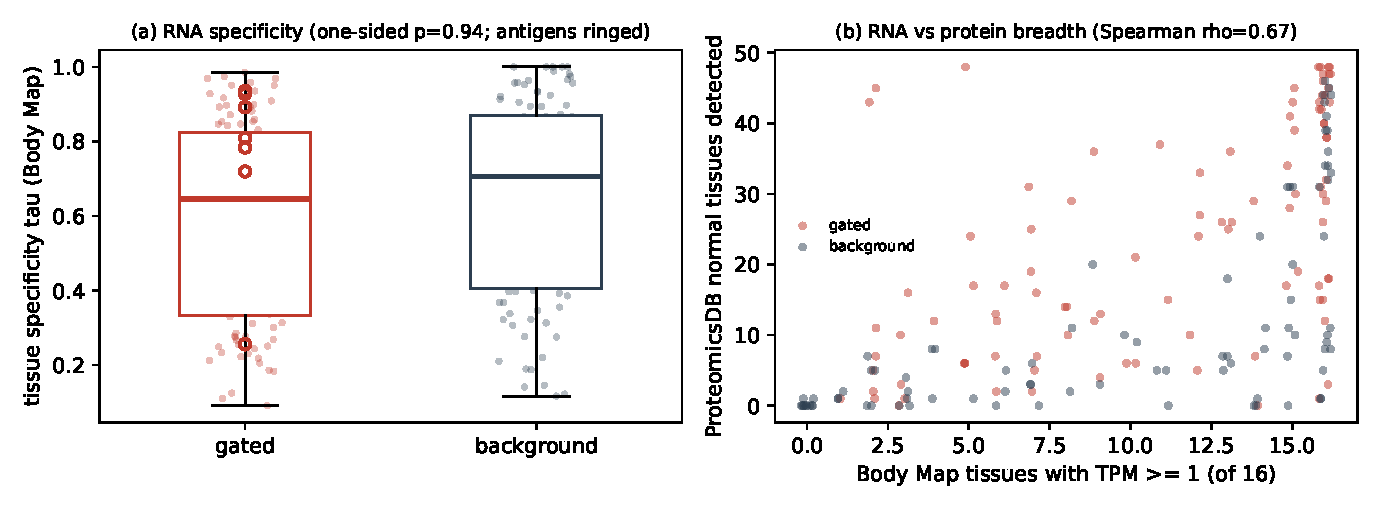
\includegraphics[width=0.95\columnwidth]{expression_atlas_fig.pdf}
\caption{Expression Atlas E-MTAB-513 audit. (a) Tissue-specificity index
$\tau$ for gated versus background genes, antigens ringed (H1, falsified).
(b) Per-gene RNA tissue breadth versus ProteomicsDB protein tissue
breadth (H2, confirmed).}
\label{fig:eatlas}
\end{figure}
